\section{The observable and the crossing limit}
\label{sec:observable}

We construct an observable with a boundary coefficient equal to the
desired crossing probability, and use bulk transport to prove that its
limit is holomorphic.

We first identify the free crossing limit on disks approximating a
polygonal Jordan quadrilateral. We then compare those crossings with the
closed-cell event in an arbitrary Jordan domain. All random discrete
domains in this section are chosen from the point geometry, independently
of the colors.

\subsection{Discrete disks and the closing star}

\begin{lemma}[Ordered polygonal approximation]
\label{lemma:polygonal-disks}
Let $D$ be a polygonal Jordan domain with finitely many marked boundary
points in their cyclic order. With probability tending to one, the
Delaunay triangulation contains a simple primal cycle whose boundary and
selected marked vertices converge to the marked boundary of $D$ in order
and in Fr\'echet distance. The triangulation inside this cycle agrees with
the full-plane triangulation on every fixed compact subset of $D$ for
all sufficiently fine good approximations.
\end{lemma}

\begin{proof}
On fine mesh in a fixed collar of $\partial D$, record the successive
Voronoi cell sites met during one traversal of $\partial D$ and join
successive sites by primal edges. A fixed polygon meets cell switches
generically almost surely. Equivalently, one can use walks through the
nearby triangles. This produces a closed primal walk, with sites and
edges uniformly close to the boundary position at the corresponding
traversal times. Its winding about a fixed interior point is one.

Extract return loops and contract them to obtain the oriented
simple-cycle decomposition of this walk. Winding is additive, so retain
a cycle with positive winding about the interior point, retaining the
original cyclic times of its edges. Every dropped interval of times has
endpoints whose physical positions tend together. Boundary simplicity
then forces its parameter length to tend to zero, unless it tends to a
whole turn. The latter possibility would put all retained times, and
thus the retained cycle, in a shrinking neighborhood of one boundary
point, contradicting its positive winding about the fixed interior
point. Hence the retained cycle follows the boundary in its order, and
marked vertices can be selected at the desired parameters. Finite
deterministic tie-breaking makes the choice measurable. Filling the
cycle by its interior triangles gives the required disk. The mesh and
local-determination estimates ensure agreement on interior compacts.
Taking a deterministic sequence of decreasing tolerances gives the
claimed convergence in probability.
\end{proof}

Fix such a disk, and initially retain only the three marked vertices
$v_0,v_1,v_2$ approximating $a,c,d$, respectively, in positive order.
Indices in the fan construction are taken modulo three. Add an exterior
vertex $s_i$ fanned to the inclusive boundary arc $v_i v_{i+1}$, add the
junction triangles $s_{i-1}s_i v_i$, and close the exterior by a triangle
$t_*$ with vertices $s_0,s_1,s_2$. This is a simple triangulation of the
sphere. Give the added vertices independent fair colors, as for the
original disk sites. No Euclidean weights on the exterior triangles are
needed.

At the closing star $t_*$, let $n_i$ be a point on the dual spoke crossing
$s_{i-1}s_i$, and assign it the label $w_i=\om^i$. This order is
\emph{opposite} to the positive cyclic order at $t_*$. For a probe $m$ in
the interior of a dual edge, define, conditionally on the geometry $\eta$,
\begin{equation}
 F_m^\eta=4\sum_{i=0}^2w_iK(m,n_i)
          =4\Esp\bigl[w_*H_{\lambda_*}(m)\bigr].
 \label{observable:definition}
\end{equation}
In the second expression, if $t_*$ is occupied by an ordinary wall, let
$i$ be its missing port and let $\lambda_*$ be that wall together with
the component reached through the missing port; set $w_*=w_i$. Set the
entire contribution to zero if $t_*$ is unused. To verify the equality,
observe that a wall not using $t_*$ has identical component indicators at
all three $n_i$, and its contribution is killed by $\sum_iw_i=0$.
The observable is constant along the interior of a dual edge, so we also
write $F_e^\eta$ for its value at a primal edge $e$. In the physical disk
the dual probe can be chosen at the intersection with that side.

Figure~\ref{fig:closing-fans} shows the completion and the boundary
pairing used below. The kernel definition is adapted to orthogonality;
its alternative description as a mean partner label will give positivity
and identify the crossing coefficient.

\begin{figure}[htbp]
\centering
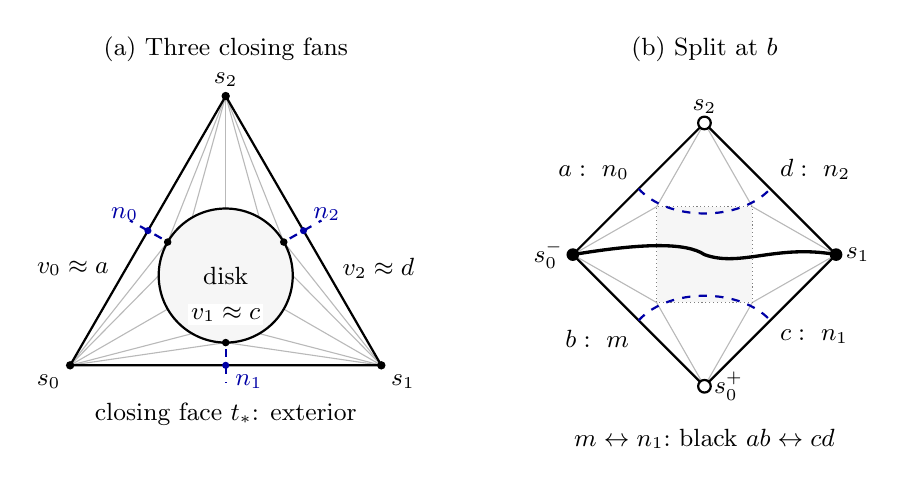
\begin{tikzpicture}[scale=.76, every node/.style={font=\small}]
\begin{scope}
 \coordinate (s0) at (-2.6,-1.5);
 \coordinate (s1) at (2.6,-1.5);
 \coordinate (s2) at (0,3);
 \fill[gray!7] (0,0) circle (1.12);
 \foreach \ang in {150,180,210,240,270}
   \draw[gray!55] (s0)--(\ang:1.12);
 \foreach \ang in {270,300,330,360,390}
   \draw[gray!55] (s1)--(\ang:1.12);
 \foreach \ang in {30,60,90,120,150}
   \draw[gray!55] (s2)--(\ang:1.12);
 \draw[thick] (s0)--(s1)--(s2)--cycle;
 \draw[thick] (0,0) circle (1.12);
 \foreach \pos in {150,270,30}{
   \fill (\pos:1.12) circle (1.8pt);
 }
 \node[anchor=east,fill=white,inner sep=1pt] at (-1.9,.12) {$v_0\approx a$};
 \node[fill=white,inner sep=1pt] at (0,-.65) {$v_1\approx c$};
 \node[anchor=west,fill=white,inner sep=1pt] at (1.9,.12) {$v_2\approx d$};
 \fill (s0) circle (2pt) node[below left] {$s_0$};
 \fill (s1) circle (2pt) node[below right] {$s_1$};
 \fill (s2) circle (2pt) node[above] {$s_2$};
 \node at (0,0) {disk};
 \draw[blue!65!black,dashed,thick] (-1.07,.62)--(-1.60,.92);
 \draw[blue!65!black,dashed,thick] (0,-1.23)--(0,-1.80);
 \draw[blue!65!black,dashed,thick] (1.07,.62)--(1.60,.92);
 \fill[blue!65!black] (-1.3,.75) circle (1.7pt)
   node[above left] {$n_0$};
 \fill[blue!65!black] (0,-1.5) circle (1.7pt)
   node[below right] {$n_1$};
 \fill[blue!65!black] (1.3,.75) circle (1.7pt)
   node[above right] {$n_2$};
 \node[align=center] at (0,-2.32) {closing face $t_*$\text{: exterior}};
 \node at (0,3.78) {(a) Three closing fans};
\end{scope}
\begin{scope}[xshift=8.0cm,yshift=.35cm]
 \coordinate (l) at (-2.2,0);
 \coordinate (r) at (2.2,0);
 \coordinate (u) at (0,2.2);
 \coordinate (v) at (0,-2.2);
 \fill[gray!7] (-.8,-.8) rectangle (.8,.8);
 \draw[gray!55] (l)--(-.8,.8) (l)--(-.8,-.8)
   (v)--(-.8,-.8) (v)--(.8,-.8)
   (r)--(.8,-.8) (r)--(.8,.8)
   (u)--(.8,.8) (u)--(-.8,.8);
 \draw[thick] (l)--(v)--(r)--(u)--cycle;
 \draw[gray,densely dotted] (-.8,-.8) rectangle (.8,.8);
 \draw[very thick] (l) .. controls (-1,.20) and (-.3,.20) .. (0,0)
    .. controls (.6,-.22) and (1.2,.18) .. (r);
 \draw[blue!65!black,dashed,thick] (-1.1,-1.1)
    .. controls (-.6,-.55) and (.6,-.55) .. (1.1,-1.1);
 \draw[blue!65!black,dashed,thick] (-1.1,1.1)
    .. controls (-.6,.55) and (.6,.55) .. (1.1,1.1);
 \foreach \p in {l,r} \fill (\p) circle (3pt);
 \foreach \p in {u,v} \draw[fill=white,thick] (\p) circle (3pt);
 \node[left] at (l) {$s_0^-$};
 \node[right] at (r) {$s_1$};
 \node[above] at (u) {$s_2$};
 \node[right] at (v) {$s_0^+$};
 \node[above left] at (-1.1,1.1) {$a:\ n_0$};
 \node[below left] at (-1.1,-1.1) {$b:\ m$};
 \node[below right] at (1.1,-1.1) {$c:\ n_1$};
 \node[above right] at (1.1,1.1) {$d:\ n_2$};
 \node[align=center] at (0,-3.08) {$m\leftrightarrow n_1$:\ black $ab\leftrightarrow cd$};
 \node at (0,3.43) {(b) Split at $b$};
\end{scope}
\end{tikzpicture}
\caption{The closing construction and one of the two boundary pairings.
In (a), the unbounded face of the drawing is the closing triangle on the
sphere; the dashed segments indicate its dual spokes. Thus the labels
$n_0,n_1,n_2$ run opposite to the positive order at its dual star.
In (b), splitting $s_0$ produces black fans on $ab,cd$ and white fans on
$bc,da$. The labels indicate the attachments of the four boundary
switches. Dashed strands show the pairing $m$--$n_1$, $n_0$--$n_2$;
the solid black path shows the corresponding connection of the black
fans. In (b), only the exterior colors are prescribed; all original disk
vertices remain free. The drawings are topological schematics.}
\label{fig:closing-fans}
\end{figure}

\par\ifdim\dimexpr\pagegoal-\pagetotal\relax<6\baselineskip\newpage\fi
\begin{proposition}[Triangular observable and the crossing coefficient]
\label{prop:observable}
The value $F_m^\eta$ belongs to the closed triangle with vertices
$w_0,w_1,w_2$. At a fan probe $s_i u$, where $u$ is interior to the boundary
arc $v_i v_{i+1}$, it belongs to the side $[w_i,w_{i+1}]$. For $i=0$ and
$u$ the marked vertex approximating $b$, the coefficient of $w_1$ on this
side is exactly the free black vertex crossing probability between the
arcs approximating $ab$ and $cd$ in the original disk.
\end{proposition}

\begin{proof}
Start with the uniform edge-pattern ensemble having oddness at $t_*$ and
$m$, and move the star defect to $n_i$ as in the proof of
\eqref{fields:orthogonal}. If the star has degree one, the loop count is
independent of the chosen port. If it has degree three, the extra loop
count is the indicator that the exterior partner of $m$ is port $i$:
joining the other two star ports creates exactly that extra loop.
Degree three has probability $1/4$. Indeed, toggling a fixed defect path
bijects to the even ensemble, whose four local even patterns at the star
are equiprobable. The port-independent terms cancel in the weighted
sum, and the factor four in \eqref{observable:definition} cancels this
probability. Thus $F_m^\eta$ is the mean partner label conditional on
degree three, proving the triangular convex-combination assertion.

For a fan probe $s_i u$, split $s_i$ into two exterior vertices, fanned
respectively to the two successive subarcs, both containing $u$, and add
the triangle formed by these two vertices and $u$. Remove $t_*$ and
prescribe alternating colors, in one fixed convention, on the four
exterior vertices now present. Leave all original disk spins free. The
four boundary edges joining consecutive exterior vertices are switches.
Their disagreement strands have the preceding conditional pairing law.

Here is the parity correspondence explicitly. The two half-edge values
at the old probe, with oddness there, have exactly one occupied half.
They become the two spoke values entering the added triangle, which has
even parity because its split exterior boundary edge is occupied. The
other three occupied exterior boundary edges are the three forced
switches at the old degree-three star. This gives a bijection from the
conditional edge-pattern ensemble to parity-even disagreement data on
all triangles of the augmented disk, with the four boundary switches
fixed. Triangle parity gives cycle parity, so the data recover colors up
to a global flip. Fixing the alternating exterior convention removes
that flip, leaving exactly uniform independent colors on all original
disk vertices.

The four switches have a noncrossing pairing. The split switch can
therefore be paired only with port $i$ or port $i+1$, proving the side
constraint. For $i=0$ at $u\approx b$, prescribe the exterior vertices
along $ab$ and $cd$ to be black, and the other two to be white. Connecting
the two black exterior vertices is equivalent to a black crossing in the
original disk: any connection between the two black fans contains a path
of original black vertices between their respective arcs, and conversely
such a path joins the fans. Pairing the split switch with port $1$ gives
this connection along the neighboring black sites. The other pairing
joins the opposite white pair, and the two possibilities are exclusive
by planarity. This proves the stated coefficient identity.
\end{proof}

\subsection{Annealed compactness for geometry-selected probes}

On failed disk-approximation events, extend all observables by arbitrary
bounded values. Those events have vanishing probability and will not
affect a limit. Original disk spins are always coupled to the fair
full-plane site colors.

The admissible probes in this subsection and below are original disk
edges, located at their physical midpoints, and fan edges $s_i u$,
located at their disk attachments $u$. A geometry-selected probe tends
to a fixed point when its location converges in probability to that
point.

\begin{lemma}[Probe compactness]
\label{lemma:probe-compactness}
From every microscopic sequence one can select a subsequence, still
satisfying the bulk transport conclusion, on which the annealed
observables converge to a continuous function $F$ in $D$ and on its three
open boundary arcs. The convergence holds for every geometry-measurable
choice of admissible probes tending to a specified point off the three
marks. The limit takes values in the closed triangle and has the
corresponding closed side values on the
open boundary arcs.
\end{lemma}

\begin{proof}
We use the ordinary-wall representation in
\eqref{observable:definition}. A nonisolated selected component has a rim
using the exterior edge $s_{i-1}s_i$, followed by a path of original disk
sites between attachments to the two different boundary arcs of those
fans. The third exterior vertex has the opposite color and cannot lie on
this rim. The disk path can degenerate to the common endpoint of its two
arcs. The component indicator tests the component side of the rim,
including its rim edges: an open dual edge belongs to that component
exactly when it is incident to an untouched triangle on the filled disk
side. An isolated selected component contributes zero at the probes in
use.

For two nearby bulk probes, different indicators force a selected-rim
visit between them. Such a visit gives a monochromatic path of original
disk sites from their neighborhood to a fixed positive distance, since
the disk portion reaches the boundary. Near a boundary point off the
three marks, compare a fan probe first with its attached disk vertex.
Unless that vertex lies on the rim, following its incident fan edge to
the vertex tests the same side; if it does lie on the rim, the required
visit already occurs. Uniform closed-disk Jordan charts join nearby disk
positions tending to the same boundary point by paths of vanishing
diameter inside the closed approximating disk. Thus a difference again
forces a nearby visit by the disk portion of the selected rim. Its two
attachments lie on different marked arcs and cannot both approach this
nonmark boundary point. One direction of the disk path therefore reaches
a fixed positive distance \emph{among original disk sites}. The exterior
fan edges do not replace this arm.

More precisely, on a fixed compact set off the marks choose a positive
distance $\rho$ valid for these continuations. For probes in a small
neighborhood of diameter $s$, choose a deterministic enlarged
neighborhood containing their short comparison paths on good geometry.
Let $q_{s,\rho}(\eta)$ be the conditional probability of a monochromatic
arm of either color from that neighborhood to distance $\rho$, under the
full-plane independent site colors. Then, for every pair of admissible
geometry-selected probes in that neighborhood, the same test gives
\begin{equation}
             |F_m^\eta-F_{m'}^\eta|
                    \le4q_{s,\rho}(\eta).
 \label{observable:conditional-arm}
\end{equation}
There is no union bound over the chosen edges. The disk and chart control
needed for this statement follows along every deterministic sequence of
good marked Jordan approximations by closed Jordan convergence; mesh
control transfers edges to their sites. Taking expectations and using
the ordinary one-arm estimate gives an upper limit tending to zero as
$s\downarrow0$. The geometry errors vanish first at fixed $s$.

Choose near-position representative edges at a countable dense set of
interior points, and fan representatives at a countable dense set of each
open boundary arc. These choices exist with vanishing location error on
good geometry. Boundedness permits a diagonal subsequence of their
annealed expectations. Estimate~\eqref{observable:conditional-arm}
extends the resulting function continuously and identifies the same
limit for all geometry-selected probes converging to any such point.
The triangle and side constraints pass to this limit by
Proposition~\ref{prop:observable}. All choices are made after the
universal bulk subsequence, so the transport conclusions remain valid.
\end{proof}

\subsection{Holomorphy without separating geometry and colors}

\begin{proposition}[Holomorphy]
\label{prop:holomorphy}
Every limit $F$ in Lemma~\ref{lemma:probe-compactness} is holomorphic in
$D$.
\end{proposition}

\begin{proof}
For a smooth compactly supported bulk test $f$, orthogonality against the
closing star, with its reversed labels, gives the exact conditional
identity
\[
                 \Esp[w_*U_{\lambda_*}(f)]=0.
\]
Indeed, at every bulk triangle the weighted sum
$\sum_j\om^jF_{m_j(t)}^\eta$ is zero by
\eqref{fields:orthogonal}. The selected nonisolated rim reaches the
exterior and therefore leaves every sufficiently small fixed test
collar. An isolated selected pair tags only exterior triangles. Apply
\eqref{transport:bulk}, partitioning $f$ into local disk tests when
needed. Its residual at the selected label tends to zero in probability
and in mean: its absolute value is bounded by the full residual
$\ell^2$ norm, which is bounded in $L^2$ by \eqref{fields:energy}.
Since
\[
 U=(1-a)V-(Q-aV),\qquad a\ne1,
\]
we obtain $\EE[w_*V_{\lambda_*}(f)]\to0$. On high-probability geometry
events the discrete disk agrees with the full triangulation throughout
the test collars; the conditional identities hold on each such graph.
The energy moments remove the omitted geometry.

Using \eqref{observable:definition} and $\sum_jd_{tj}=0$, we have therefore
proved
\begin{equation}
 \EE\left[\sum_t f(z_t)\sum_jd_{tj}F_{m_j(t)}^\eta\right]
                          \longrightarrow0.
 \label{observable:discrete-cr}
\end{equation}
The edge coefficients and the conditional observable both depend on the
point geometry, so their product cannot be replaced by a product of
expectations. We instead express the edge coefficients as a random
measure and prove that this measure has a deterministic limit.

Group the two contributions of each shared edge $e=t\cap t'$. If $d_{t,e}$
is its clockwise side vector for $t$, set
\[
 \mu_\eps=\sum_e d_{t,e}\bigl(f(z_t)-f(z_{t'})\bigr)\delta_{m_e},
\]
where now $m_e$ denotes the physical midpoint of the side. This weight is
independent of which adjacent triangle is called $t$. All edges involved
are buffered inside the disk. Let $T_\eps(B)=|\mu_\eps|(B)$.
Because $f$ is smooth,
\[
 |d_{t,e}|\,|f(z_t)-f(z_{t'})|
 \le C_f\bigl(\diam(t)^2+\diam(t')^2\bigr).
\]
Consequently, for each sufficiently small fixed square $B$ of side $s$
in a compact bulk neighborhood,
\begin{equation}
        \limsup_{\eps\to0}\|T_\eps(B)\|_2\le C_fs^2.
 \label{observable:variation}
\end{equation}
The triangles incident to an edge assigned to $B$ lie in a fixed
enlargement on fine mesh; the exceptional contribution is controlled by
their higher moments.

For a deterministic smooth function $G$, midpoint integration on
clockwise triangle boundaries gives
\[
 \mu_\eps(G)
 \longrightarrow -\int_D f\,\dd G\wedge\dd z
              =\int_DG\,\dd f\wedge\dd z
                 \quad\text{in }L^1\text{ of the geometry}.
\]
To check the approximation, the midpoint error on a triangle is
$O_{f,G}(\diam(t)^3)$. The sum of these errors tends to zero in $L^1$,
using the maximum mesh diameter times the bounded diameter-square sum.
Stokes' theorem, the clockwise orientation, and area approximation give
the displayed sign. Replacing $f(z_t)$ by $f$ in each triangle has the
same vanishing cubic-error bound. The resulting limiting complex measure
is
\[
                     \mu=\dd f\wedge\dd z,
\]
which has a bounded compactly supported density.

We need the stronger conclusion for fixed-square indicators. If $B$ is
such a square, choose a smooth $g_\tau$ with $0\le g_\tau\le1$ agreeing
with $\ind_B$ outside a boundary strip $U_\tau$ of width $O(\tau)$. Then
\[
 |\mu_\eps(B)-\mu(B)|
 \le |\mu_\eps(g_\tau)-\mu(g_\tau)|
                   +T_\eps(U_\tau)+|\mu|(U_\tau).
\]
Cover $U_\tau$ by $O(\operatorname{perimeter}(B)/\tau+1)$ squares of
side $O(\tau)$. The first-moment consequence of
\eqref{observable:variation}, after the microscopic limit, makes the
expected variation on this strip $O_f(\operatorname{perimeter}(B)\tau+
\tau^2)$. The limiting variation tends to zero there as well. First take
$\eps\to0$, then $\tau\downarrow0$, obtaining
\begin{equation}
                W_\eps(B):=\mu_\eps(B)\longrightarrow
                w(B):=\mu(B)\quad\text{in }L^1.
 \label{observable:square-l1}
\end{equation}

Now fix a deterministic tiling of the test neighborhood by squares of
side $s$, and choose a conditional representative $F_B^\eta$ on an edge
near the center of each square. The same ordinary arm test in
\eqref{observable:conditional-arm} controls every edge assigned to $B$:
\[
 |F_e^\eta-F_B^\eta|\le4q_B(\eta),\qquad
 \limsup_{\eps\to0}\EE q_B\le C(s/\rho)^c,
 \qquad 0\le q_B\le1.
\]
Here $\rho>0$ is fixed by the distance of the support neighborhood to the
boundary. Thus $\EE q_B^2\le\EE q_B$, and without an independence
assumption Cauchy--Schwarz gives
\[
 \limsup_{\eps\to0}\EE[T_\eps(B)q_B]
      \le C_{f,\rho}s^{2+c/2}.
\]
Summing over $O(s^{-2})$ squares bounds the mean replacement error by
$C_{f,\rho}s^{c/2}$. For fixed $s$, omitted geometry contributes a
vanishing mean by boundedness of the observable and the variation
moments.

At this fixed tiling, \eqref{observable:square-l1} can be multiplied by
the correlated representative because $|F_B^\eta|\le1$:
\[
 \left|\EE[F_B^\eta W_\eps(B)]-w(B)\EE F_B^\eta\right|
 \le\EE|W_\eps(B)-w(B)|\longrightarrow0.
\]
Lemma~\ref{lemma:probe-compactness} identifies
$\EE F_B^\eta\to F(\operatorname{center}(B))$. Hence
\eqref{observable:discrete-cr}, followed first by $\eps\to0$ at fixed
tiling and then by $s\downarrow0$, yields
\begin{equation}
                       \int_D F\,\dd f\wedge\dd z=0
                       \qquad(f\in C_c^\infty(D)).
 \label{observable:cr}
\end{equation}
Since $\dd f\wedge\dd z=2\ii\,\partial_{\bar z}f\,\dd^2z$, this is
the distributional Cauchy--Riemann equation. Local mollification and
continuity of $F$ show that $F$ is holomorphic.
\end{proof}

\subsection{The three boundary arcs determine the conformal map}

The three closed sides of a nondegenerate triangle have empty common
intersection. The side constraints therefore show that $F$ is
nonconstant. The open mapping theorem puts its interior values in the
open equilateral triangle. Conformal charts for the polygon and the
triangle, with their Carath\'eodory boundary extensions, reduce the
remaining uniqueness issue to the following lemma.

\par\ifdim\dimexpr\pagegoal-\pagetotal\relax<6\baselineskip\newpage\fi
\begin{lemma}[Boundary uniqueness]
\label{lemma:boundary-uniqueness}
Let $G:\mathbb D\to\mathbb D$ be nonconstant and holomorphic. Let
$\zeta_0,\zeta_1,\zeta_2$ and $\eta_0,\eta_1,\eta_2$ be positively
ordered triples of distinct points of the unit circle. Suppose that $G$
extends continuously to each open arc $(\zeta_i,\zeta_{i+1})$ and takes
its values there in the corresponding positively oriented closed arc
$[\eta_i,\eta_{i+1}]$. Then $G$ extends continuously to the closed disk,
maps $\zeta_i$ to $\eta_i$, and is a conformal bijection of the disk.
\end{lemma}

\begin{proof}
On each open source arc, Schwarz reflection across the unit circle
extends $G$ holomorphically across the boundary. Near each point of that
arc, $G$ is nonzero, so $u=\log|G|$ is harmonic, negative on the disk
side, and zero on the circle. The Hopf boundary lemma and the
Cauchy--Riemann equations give
\[
 \frac{\dd}{\dd t}\arg G(e^{\ii t})
    =\left.\frac{\partial}{\partial r}\log|G(re^{\ii t})|\right|_{r=1}
    >0.
\]
The proper target arc has a bounded real argument lift. Thus the
boundary argument on each open source arc is strictly increasing and
has finite one-sided limits at its endpoints.

We prove that the two limits at a source mark agree, without assuming
interior continuity there. Rotate that mark to $1$ and denote the limits
as $t\uparrow0$ and $t\downarrow0$ by $L_-$ and $L_+$, respectively.
Let $g(e^{\ii t})$ be the known boundary values, with arbitrary values
assigned at the three marks. For fixed $z\in\mathbb D$, Cauchy's formula
on a circle of radius $R>|z|$ is
\[
 G(z)=\frac1{2\pi}\int_{-\pi}^{\pi}
       \frac{G(Re^{\ii t})}{1-(z/R)e^{-\ii t}}\,\dd t.
\]
As $R\uparrow1$, the numerator converges away from the three marks and
is uniformly bounded, while the denominator stays uniformly away from
zero for this fixed $z$. Dominated convergence therefore gives
\[
 G(r)=\frac1{2\pi}\int_{-\pi}^{\pi}
                 \frac{g(e^{\ii t})}{1-re^{-\ii t}}\,\dd t,
                 \qquad 0<r<1.
\]
For a fixed small $\alpha>0$, write $\ell_r=\log(1/(1-r))$. The
logarithmic primitive of the kernel gives
\[
 \int_0^\alpha\frac{\dd t}{1-re^{-\ii t}}
       =\frac{\ell_r}{\ii}+O_\alpha(1),\qquad
 \int_{-\alpha}^0\frac{\dd t}{1-re^{-\ii t}}
       =-\frac{\ell_r}{\ii}+O_\alpha(1).
\]
For example, a continuous branch of
$\ii^{-1}\log(e^{\ii t}-r)$ is a primitive on either interval.
Moreover, the kernel is bounded in modulus by
$C/(1-r+|t|)$ there. Replacing $g$ by its corresponding one-sided
limit therefore gives an $o(\ell_r)$ error: for every $\delta>0$ choose
a smaller fixed interval where $|g-L_\pm|<\delta$, use the logarithmic
kernel bound on that interval, and note that the complementary fixed
interval has a bounded integral as $r\uparrow1$. Then let $\delta$ tend
to zero. The part away from the mark is also bounded. Consequently,
\begin{equation}
 G(r)=\frac{L_+-L_-}{2\pi\ii}\log\frac1{1-r}
            +o\!\left(\log\frac1{1-r}\right).
 \label{observable:jump}
\end{equation}
Boundedness of $G$ forces $L_+=L_-$. The common value belongs to the two
adjacent target arcs, whose intersection is their prescribed common
endpoint; hence $G$ has the required continuous circle trace $g$.

To obtain continuity for all interior approaches, apply the same
radial-circle limiting argument to the Poisson formula for the bounded
harmonic real and imaginary parts of $G$. They are the Poisson
extensions of the continuous circle trace $g$. The Poisson extension of
continuous circle data is continuous on the closed disk. In particular,
this proves full continuity at the marks, not merely radial or
nontangential convergence.

On each open arc the boundary argument increases strictly between the
two prescribed consecutive endpoints. The boundary curve therefore
traverses the circle once in positive order. For any $w\in\mathbb D$,
continuity on the closed disk gives uniform convergence of
$G(re^{\ii t})-w$ to $g(e^{\ii t})-w$ as $r\uparrow1$. The winding number
is one for all sufficiently large $r$. The argument principle gives
exactly one zero of $G-w$ in $|z|<r$, counted with multiplicity. Letting
$r\uparrow1$ proves that every $w$ has exactly one preimage, of
multiplicity one. Thus $G$ is a conformal bijection.
\end{proof}

It follows that $F$ is the conformal map to the equilateral triangle with
$a,c,d$ mapped to $w_0,w_1,w_2$. Normalize a conformal map to the upper
half-plane by
\[
                  (a,b,c,d)\longmapsto(0,x,1,\infty),\qquad 0<x<1.
\]
The Schwarz--Christoffel integral for three angles $\pi/3$ gives the
proportion along the side from $w_0$ to $w_1$ at $b$ as
\begin{equation}
 \mathcal C(x)=
 \frac{\displaystyle\int_0^x u^{-2/3}(1-u)^{-2/3}\,\dd u}
      {\displaystyle\int_0^1 u^{-2/3}(1-u)^{-2/3}\,\dd u}.
 \label{observable:beta}
\end{equation}
By Proposition~\ref{prop:observable}, this is the limiting annealed
coefficient of $w_1$ at the fan probe for $b$, and therefore the limiting
free black vertex crossing probability. Every microscopic sequence has
a further subsequence with this same limit. Since the crossing
probabilities are bounded, their full sequence converges to
$\mathcal C(x)$ on the discrete polygonal disks.

\subsection{The closed-cell event in every Jordan domain}

\begin{proposition}[Fixed-buffer Jordan comparison]
\label{prop:jordan-squeeze}
Let $D$ be any bounded Jordan domain with distinct positively ordered
boundary marks $a,b,c,d$. For the full-plane Poisson tessellation with
independent fair cell colors, the annealed probability of a connected
crossing in the closed black-cell union intersected with $\overline D$,
from $ab$ to $cd$, converges to $\mathcal C(x)$ with the marked conformal
parameter of $D$.
\end{proposition}

\begin{proof}
Choose an orientation-preserving plane Jordan--Schoenflies homeomorphism
$\Phi$ taking $\overline D$ to $[0,1]^2$, with the target arcs $ab$ and
$cd$ going to the left and right sides. For fixed $0<\delta<1/8$, define
in these coordinates the harder and easier rectangles
\[
 R^-_\delta=[-\delta,1+\delta]\times[\delta,1-\delta],
 \qquad
 R^+_\delta=[\delta,1-\delta]\times[-\delta,1+\delta].
\]
The first rectangle lengthens a horizontal crossing while restricting
its height; the second shortens the crossing and allows more height.
Figure~\ref{fig:jordan-buffers} displays these two comparisons.
Approximate their inverse images under $\Phi$ by deterministic polygonal
marked quadrilaterals, in their boundary order and much more accurately
than the buffer margins. For each of the two polygons use the discrete
disks from Lemma~\ref{lemma:polygonal-disks}. Their original vertices
inherit the full-plane free colors, so the crossing results already
proved apply to them.

\begin{figure}[htbp]
\centering
\begin{tikzpicture}[scale=3.7,every node/.style={font=\small}]
 \begin{scope}
  \fill[gray!7] (0,0) rectangle (1,1);
  \draw[gray] (0,0) rectangle (1,1);
  \draw[very thick] (0,0)--(0,1) (1,0)--(1,1);
  \draw[blue!65!black,thick] (-.14,.14) rectangle (1.14,.86);
  \draw[blue!65!black,thick,-{Stealth[length=4pt]}]
    (-.14,.48) .. controls (.20,.65) and (.65,.32) .. (1.14,.55);
  \node[below left] at (0,0) {$0$};
  \node[below right] at (1,0) {$1$};
  \node[blue!65!black,above] at (.5,.86) {$R^-_\delta$};
  \node at (.5,1.23) {Harder crossing};
  \node[align=center] at (.5,-.31) {wider and shorter};
 \end{scope}
 \begin{scope}[xshift=2.0cm]
  \fill[gray!7] (0,0) rectangle (1,1);
  \draw[gray] (0,0) rectangle (1,1);
  \draw[very thick] (0,0)--(0,1) (1,0)--(1,1);
  \draw[blue!65!black,thick] (.14,-.14) rectangle (.86,1.14);
  \draw[thick,-{Stealth[length=4pt]}]
    (0,.40) .. controls (.30,.65) and (.65,.32) .. (1,.57);
  \node[below left] at (0,0) {$0$};
  \node[below right] at (1,0) {$1$};
  \node[blue!65!black,above] at (.5,.76) {$R^+_\delta$};
  \node at (.5,1.23) {Easier crossing};
  \node[align=center] at (.5,-.31) {narrower and taller};
 \end{scope}
\end{tikzpicture}
\caption{Fixed buffers in the coordinates of $\Phi$. The gray square is
$\Phi(\overline D)$, with its two target sides in bold; the blue boundary
is the comparison rectangle. A path crossing the harder rectangle
contains a crossing of the square, while a path crossing the square
contains a crossing of the easier rectangle. Strict margins preserve
these implications under the
polygonal and discrete approximations. The picture is in square
coordinates and imposes no metric regularity on the physical Jordan
boundary or on the chart.}
\label{fig:jordan-buffers}
\end{figure}

Keep all these choices fixed while taking $\eps\to0$. Work on the
high-probability event of the needed disk approximation and mesh control
in a fixed compact neighborhood. Both $\Phi$ and $\Phi^{-1}$ are uniformly
continuous on the relevant compact sets. Thus any fixed coordinate
margin is preserved by taking the physical polygonal and mesh errors
sufficiently small. No Lipschitz estimate for either chart is required.

\paragraph{The harder crossing implies a closed-cell crossing.}
A black primal vertex crossing of the harder disk gives a continuous
black-cell path: for each successive pair of neighboring sites, join
them through their shared Voronoi side, with the two segments lying in
the two closed black cells. Mesh control keeps this path uniformly close
to the primal path. In square coordinates it stays in a height band
strictly inside $(0,1)$, starts to the left of $x=0$, and ends to the
right of $x=1$. Take its first contact with $x=1$ and the last preceding
contact with $x=0$. Between those times its first coordinate lies in
$[0,1]$, and its height remains in $(0,1)$. This clipped path is therefore
a crossing of $\overline D$ in the closed black-cell union.

\paragraph{A connected closed-cell crossing gives a finite primal chain.}
First recall local finiteness, including cells whose nuclei lie outside
the region of interest. On a fixed compact neighborhood, the distance
to the nearest site has a finite maximum: a finite cover, or comparison
with any fixed site, gives such a bound. A cell meeting that neighborhood
has its nucleus within the resulting bounded enlargement. Poisson local
finiteness therefore leaves only finitely many such cells.

If a connected crossing set is not closed, take its closure. The black
cell union is closed locally, being a locally finite union of closed
cells. The closure consequently remains black, connected, and contained
in $\overline D$, and retains its contacts with both target arcs. Denote
this compact connected set by $K$. For every black cell $C_j$ meeting
$K$, let $E_j=K\cap C_j$. These finitely many nonempty relatively closed
sets cover $K$. Their incidence graph is connected: a partition into two
nonempty collections with no intersecting members would express $K$ as
the disjoint union of two relatively closed sets, a separation. Hence
there is a finite touching chain of black cells from a left-contact cell
to a right-contact cell.

Cells meeting along a Voronoi edge have neighboring sites. If two cells
meet only at a Voronoi vertex, Poisson general position gives exactly
three cells there, with nuclei forming a Delaunay triangle; those two
sites are again neighbors. Thus the touching chain yields a black
full-plane primal vertex chain, also for the vertex-only contacts
permitted by the closed-cell event. Fine mesh makes its nuclei and edges
arbitrarily close to $K$. For an edge of the chain, use its cell-contact
point in $K$: both neighboring nuclei lie close to that point, and so
does their straight Delaunay edge. This justifies the proximity without
any convexity assumption on $D$.

\paragraph{The chain contains a crossing of the easier disk.}
In square coordinates the chain stays in a small enlargement of
$[0,1]^2$, starts strictly to the left of the easier disk, and ends
strictly to its right. Its allowed height band is disjoint from the
easier disk's entire top and bottom boundary arcs. A fixed vertical
middle strip within that band lies inside the approximating disk; its
left and right boundary-arc neighborhoods lie on opposite sides of this
strip. These assertions have strict margins, so hold for the polygonal
and discrete approximations already fixed.

\begingroup\widowpenalty=10000
The chain and the disk boundary are paths in the same planar primal
graph. They can meet only at vertices or along shared edges. The chain
has a left boundary contact before its first right boundary contact:
to reach the right side from its starting position it must pass through
the interior middle strip, and the top and bottom arcs are inaccessible.
Choose that first right contact, and then the last left contact
preceding it. Between these contacts there are no boundary visits.
Any shared boundary edge would have boundary endpoint vertices and
would also be such a visit. The intervening subpath crosses the interior
middle strip, since its endpoints lie on opposite sides. A connected
path avoiding a simple boundary cycle cannot move between its interior
and exterior. This subpath is therefore in the interior, with its two
endpoints on the left and right vertex arcs of the closed disk. Removing
repeated vertices if necessary gives its black crossing.\par
\endgroup

\paragraph{Limit order.}
Write $p^-_{\eps,\delta}$ and $p^+_{\eps,\delta}$ for the free crossing
probabilities of these fixed harder and easier discrete disks, and
$p_\eps(D;a,b,c,d)$ for the requested closed-cell probability. The two
pathwise comparisons, with the vanishing geometry exception, imply
\[
 p^-_{\eps,\delta}-o(1)
 \le p_\eps(D;a,b,c,d)
 \le p^+_{\eps,\delta}+o(1),
\]
where $\delta$ and the deterministic polygons are fixed during the
microscopic limit. The outer probabilities converge to
$\mathcal C(x^-_\delta)$ and $\mathcal C(x^+_\delta)$ by the polygonal
result. Now shrink the buffers, choosing their polygonal approximation
errors to vanish faster than their coordinate margins. The marked
boundaries converge in order and in Fr\'echet distance to the original
Jordan boundary. Closed Jordan conformal convergence gives
$x^-_\delta,x^+_\delta\to x$. Since $\mathcal C$ is continuous on
$(0,1)$, the displayed inequalities squeeze the requested limit to
$\mathcal C(x)$.
\end{proof}

Finally,
\[
 \int_0^1u^{-2/3}(1-u)^{-2/3}\,\dd u
             =\frac{\Gamma(1/3)^2}{\Gamma(2/3)},\qquad
 \int_0^xu^{-2/3}(1-u)^{-2/3}\,\dd u
             =3x^{1/3}\,{}_2F_1(1/3,2/3;4/3;x).
\]
The second identity follows by integrating the binomial series on
$[0,x]$, and $\Gamma(4/3)=\Gamma(1/3)/3$. Substitution into
\eqref{observable:beta} yields exactly \eqref{eq:cardy}. Together with
Proposition~\ref{prop:jordan-squeeze}, this proves
Theorem~\ref{thm:cardy} for the stated full-plane annealed law and the
closed-cell convention.
